% Refer to the UMD style guide for the requirements for your dissertation
% Current version (2021)
% https://gradschool.umd.edu/sites/gradschool.umd.edu/files/uploads/DissertationThesis/etd_style_guide_201708.pdf
\title{Quantum routing for architecture-respecting circuit transformations}

% \includeonly{Acknowledgements}

\begin{document}

\frontmatter
\pagestyle{empty}
\singlespacing
%Abstract Page
\hbox{\ }

\begin{center}
\large{{ABSTRACT}}

\vspace{3em}

\end{center}
\hspace{-.15in}
\begin{tabular}{ll}
Title of Dissertation:     & {\large  Many-body entanglement dynamics }\\
                           & {\large  and computation } \\
                           & {\large  in quantum systems with power-law interactions } \\
\                         \\
                           & {\large  Andrew Guo } \\
                           & {\large Doctor of Philosophy, 2022} \\
\                         \\
Dissertation Directed by:  & {\large  Professor Alexey V. Gorshkov} \\
                           & {\large  Department of Physics } \\
\end{tabular}

\vspace{3em}

% Use word count on the text file
\begin{doublespacing}
Quantum many-body systems with long-range interactions---such as those that decay as a power-law in the distance between particles---are promising candidates for quantum information processors. Due to their high degree of connectivity, they are potentially capable of generating entanglement more quickly than systems limited to local interactions, which may lead to faster computational speeds. The questions of the nature of the speed-ups they can achieve---as well as how to program these long-range systems to achieve such speed-ups---are, therefore, of prime theoretical interest.
% In this thesis, we study the nature of the speed-ups they can achieve as well as the fundamental speed limits on their dynamics.

To understand the nature of the speed-ups achievable, it is natural to consider the dual question, which is \emph{what are the fundamental speed limits in quantum many-body systems?} Given that most systems relevant to quantum computation operate in the non-relativistic regime---where information typically propagates at velocities far below the threshold set by the speed of light---the absence of an absolute speed limit seems to allow for unbounded rates of information transfer. However, in 1972, Lieb and Robinson restored a notion of locality in systems with local interactions by proving a bound that led to light-cone-like regions outside which information propagation is exponentially suppressed \cite{LR}. The question of whether similar bounds could be proven for long-range systems has remained open---until recently.

In this thesis, we will describe results related to the now-fuller picture of the fundamental rates of information propagation in power-law-interacting systems.
First, we consider the regime of ``strongly long-range'' interactions, for which velocities can grow unboundedly with system size. We will present Lieb-Robinson-type bounds for these systems and also outline a protocol that can transfer quantum states as fast as these bounds will allow. we will also discuss the implications of these bounds for quantum information scrambling.

The second part of the thesis will study how protocols for transferring quantum states quickly can be used to perform multi-qubit gates. In particular, we will demonstrate how the power of long-range interactions allows one to implement the unbounded fanout gate asymptotically faster than systems with local interactions. This result also implies the hardness of simulating the dynamics of long-range systems evolving for superlogarithmic times, and demonstrates the potential for insights from quantum many-body physics to lead to a more powerful toolbox for quantum computation.

Finally, we will address the question of fundamental speed limits in quantum systems that are open to the environment. A priori, it may seem surprising that such speed limits may exist, since non-unitary processes may break locality constraints. However, we show that under certain assumptions such as linearity and Markovianity of the bath, one can restore a notion of locality using Lieb-Robinson-type bounds. We use the resulting bounds to constrain the entanglement structure of the steady states of open long-range systems, a first step towards proving the area law for such systems.
\par
\end{doublespacing}
 %(must be first, required, non-numbered)
%Titlepage
\hbox{\ }
\vspace{1in}
\begin{center}

\large{{MANY-BODY ENTANGLEMENT DYNAMICS AND COMPUTATION IN QUANTUM SYSTEMS WITH POWER-LAW INTERACTIONS}}\\
\ \\
\ \\
\large{by} \\
\ \\
\large{Andrew Guo}%Your full name as it appears in University records.
\ \\
\ \\
\ \\
\ \\
\normalsize
Dissertation submitted to the Faculty of the Graduate School of the \\
University of Maryland, College Park in partial fulfillment \\
of the requirements for the degree of \\
Doctor of Philosophy \\
2022
\end{center}

\vspace{7.5em}

\noindent Advisory Committee: \\
Professor Alexey V.\ Gorshkov, Co-Chair/Co-Advisor \\
Professor Victor Galitski, Co-Chair
Professor Andrew M.\ Childs, Dean's Representative \\
Professor Brian Swingle, Co-Advisor\\
Professor Xiaodi Wu
 %(must follow Abstract, required, non-numbered)
% %Copyright

\thispagestyle{empty}
\hbox{\ }

\vfill

\vspace{.5in}

\begin{center}
\large{\copyright \hbox{ }Copyright by\\
Eddie Schoute  %Type your name as it appears in University records
\\
2021}
\end{center}

\vfill

\newpage 
 %(highly recommended, non-numbered)


%Pages from this point start at lower-case Roman number ii)
\pagestyle{plain}
\setcounter{page}{2}

\ifbool{doublespaced}{\doublespacing}{}
% Preface or Foreword
% Dedication
\chapter{Acknowledgments}
A Ph.D. is not easy and there's a long list of people to whom I owe a debt of gratitude. This is an incomplete list, but I will mention as many as I can.
First, my advisors and mentors through grad school, Alexey and Brian, were paragons of unquenchable curiosity and intellectual voracity. They were also extremely generous and patient, and always there to lend an ear. I thank them both for their guidance and support.

I also want to thank the postdocs with whom I've had the pleasure of learning from, including Zhe-Xuan Gong, Mike Foss-Feig, and Shenglong Xu, former graduate students Zachary Eldredge and Jeremy Young, and later my Flatiron mentors Peter Lunts, Miles Stoudenmire, and Matt Fishman. I thank my collaborators on everything Lieb-Robinson---Minh Tran, Adam Ehrenberg, and Abhinav Deshpande---and on scrambling---Tianci Zhou and Xiao Chen.

A list of postdoc mentors who lent their advice:
Chris Baldwin,
Jim Garrison,
Lucas Brady,
Luis-Pedro Garcia,
Przemek Bienias,
Simon Lieu, and
Zhicheng Yang.
A list of QuICS/JQI and CS graduate students:
Alireza Seif,
Aniruddha Bapat,
Denis Peskov,
Dhruv Devulapalli,
Eddie Schoute,
Fangli Liu,
Jon Kunjummen,
Jonathan Curtis,
Manasi Shingane,
Matt Kovacs-Deak,
Naren Manjunath,
Nhung Nguyen,
Pradeep Niroula,
Ron Belyansky,
Su-Kuan Chu,
Subhayan Sahu,
Yidan Wang,
Yuan Su, and
Yusuf Alnawaktha.

Thanks to the staff of QuICS and JQI. In particular, thanks to Javiera Caceres, Andrea Svejda, Melissa Britton for helping with travel and finances, and Josiland for helping me through the graduation paperwork.
I want to thank members of the GRAD-MAP team for working to support diversity, especially my co-leads, Milena Crnogorcevic and Charlotte Ward. Thanks to various members of the Physics and CS departments for the fun that helped preserve sanity, including board games and volleyball/frisbee, to the members of the Linke Lab who adopted me and took me along camping and beach trips, and finally to the Klein's Group of (approximately) Four: Abhinav, Ani, Eddie, and Minh, for being solid friends through thick and thin.

Along the road to this Ph.D. were the fair share of stumbles and failures. The true credit goes out to those who stayed by my side and stepped up when times were roughest. To that end, I thank my family---my mom, dad, grandma, and Vivian, as well as my extended family---for always having my back, Alexey for his patience and understanding and, of course, my beloved Yingyue Zhu, whose love and devotion has been a steadfast pillar of support throughout the good times and the bad. Thank you.
 %(if present, lower-case Roman)
\ifbool{doublespaced}{\singlespacing}{}

% \cleardoublepage
% \microtypesetup{protrusion=false} % If you use microtype
\tableofcontents %(required, lower-case Roman)
% \microtypesetup{protrusion=true}

% List of tables
% List of figures
% List of abbreviations

\newpage
\ifbool{doublespaced}{\doublespacing}{}
\mainmatter

%!TEX root = body.tex
\chapter{Introduction}

%Title
% Many-body entanglement dynamics and computation in quantum systems with power-law interactions
At the heart of every quantum computer lies a many-body quantum system. These systems can inhabit a rich and complex class of states with exotic and interesting properties in their own right. One of the fundamental properties that delineate them from classical systems is their ability to experience entanglement. Entanglement allows quantum systems to experience an extra level of correlations that extend beyond classical probability theory. These correlations provide a source of \emph{quantum} information and are what enable the performance of quantum computing. Indeed, a quantum computation can be viewed as the dynamics of a many-body system whose evolution to an entangled state encodes a computational problem. As such, the rate at which a many-body system can generate entanglement directly informs how quickly this computation can be performed in practice.

Most many-body systems relevant to modern quantum technologies can be viewed to operate in a non-relativistic regime,
%[citation needed?]
where typical velocities of information propagation are far below the threshold set by the speed of light. In this regime, an absolute speed limit is lacking due to the absence of causality inherent in the Schr\"odinger equation.
As such, a fundamental question in quantum many-body physics is, \emph{what are the fastest rates at which entanglement can spread in such systems?}

The first bounds on these rates were shown by Elliot Lieb and Derek Robinson in 1972 \cite{LR}.
Since then, much progress has been made on sharpening these bounds \cite{ChenLucas2021graphtheory,WangHazzard2020} and proving them for specific classes of systems \cite{Tran2019a,Chen2019,kuwaharaStrictlyLinearLight2020,Tran2021b}.
In addition to bounding the rate of entanglement generation, these bounds are also connected to a diverse array of phenomena, including the decay of correlations in the ground state \cite{Hastings2006}, generation of topological order \cite{Bravyi2006, Bravyi2010}, efficiency of classical/quantum simulation \cite{Osborne2006,Tran2019a}, hardness of bosonic sampling tasks \cite{Deshpande2018}, heating rates in periodically driven Floquet systems \cite{Abanin2015,Tran2019b}, and signatures of quantum chaos \cite{Lashkari2013,Guo2019}.

The ability of quantum computers to generate entanglement is central to their ability to achieve speed-ups in problems that are believed to be intractable for classical computers.
Solving hard problems quickly has been the selling point of quantum computers since 1994, when Peter Shor discovered his algorithm for fast integer factorization \cite{Shor1997}.
While in practice the computational speed of a quantum computer is inherently determined by parameters of the hardware that realizes the computer, the ``software'' can also play an important role.
In particular, the choices of algorithms and protocols used to perform the various gates and subroutines in the quantum circuit can affect the asymptotic runtimes.
% These protocols are highly dependent on the mapping between the circuit-level system and the system-level hardware.  the quantum circuits, which can affect their asymptotic runtimes.
% Choosing the right sets of gates to match the native hardware and takes best advantage of the limited resources is an important problem.
It can therefore be advantageous to study the theoretically optimal speeds of entanglement generation in more abstract models that are universal to all quantum computers, regardless of the underlying hardware.
% As such, it's important to study the theoretically optimal rates at which entanglement can be generated in these systems---to ensure that the computation takes the best advantage of the limited resources.

And in terms of the hardware, today's quantum computers are indeed quite limited. They contain small numbers of qubits that decohere quickly. Furthermore, many of the prevalent models also rely on restricted qubit layouts such as a 2D planar grid architecture \cite{Arute2019}, whereas the standard circuit model of quantum computing assumes one may apply single-qubit and two-qubit gates on arbitrary non-overlapping subsets of the qubits.
Since this assumption of being able to directly apply interactions between two arbitrarily distant qubits does not hold in practice for large quantum computing architectures \cite{Monroe2014,Linke2017,Bapat2018,Childs2019c,Bapat2022}, it leads to further overheads when mapping circuits to these restricted connectivities.
These overheads can affect the asymptotic scaling of the quantum algorithms and possibly negate their quantum advantages.
As such, it motivates the need to study both novel architectures as well as new ways of generating entanglement quickly.

In terms of novel architectures for quantum computing, systems that possess longer-range interactions provide promising candidates.
In particular, power-law interactions---those that decay as a power-law $1/r^\alpha$ in the distance  $r$ between particles, for some $\alpha > 0$---provide a natural way of augmenting the power of quantum systems.
These not-so-local interactions are native to many experimental quantum systems and include dipole-dipole and van der Waals interactions between Rydberg atoms~\cite{Saffman2010,Weimer2012}, dipole-dipole interactions between polar molecules~\cite{Yan2013}, defect centers in diamond~\cite{Yao2012,Weimer2012}, and magnetic atoms~\cite{Fraxanet2022}.
Such systems have attracted interest due to their ability to act as quantum sensors \cite{Foss-Feig15} and clocks, in addition to their potential as resources for faster quantum information processing.

Recently, Refs.~\cite{kuwaharaStrictlyLinearLight2020,Eldredge2017,Guo2020,Tran2021a} gave protocols that take advantage of power-law interactions to quickly transfer a quantum state across a lattice.
As we will show in \cref{ch:qfo}, it is also possible to leverage the power of these interactions to implement quantum gates asymptotically faster than is possible with finite-range interactions.
Furthermore, the Lieb-Robinson bounds discussed earlier that bound the rate of transferring quantum states or engineering many-body entangled states can also lead to new tools for lower-bounding the runtimes of quantum algorithms.
% And using many-body Hamiltonians, it may be possible to engineer protocols to transfer quantum states quickly---which can be used for quantum routing---or to produce many-body entangled states quickly.
% As we show in this thesis, these entangled states can be used as resources for performing certain multiqubit quantum gates quickly.
These two applications combined demonstrate the power of many-body physics to enhance the computational toolkit for quantum information scientists.

% In \cref{ch:vlr}, we provide one such demonstration of this synthesis of perspectives. We provide a set of matching upper and lower bounds for the time it takes to transfer quantum states in systems that can be mapped to free bosons or fermions hopping on a $d$-dimensional lattice with $1/r^{\alpha}$ hopping strength. Specifically, for systems with $N$ lattice sites, we prove a Lieb-Robinson-type bound of on the time required to transfer a single free boson/fermion $t \gtrsim N^{\alpha/d}/\sqrt{N}$ for $\al < d/2$ and show that it can be saturated by a new quantum state transfer protocol. We also prove a bound for many-site signaling (from one site to an extensive part of the system) that can be saturated. This bound leads to a bound on scrambling of $t_\text{sc}\gtrsim N^{\alpha/d}/N$, which generalizes the result in Ref.~\cite{Lashkari13} of $t_\text{sc} \gtrsim 1/N$ to all $\alpha<d$.

In \cref{ch:vlr}, we provide one such demonstration of this synthesis of perspectives. We provide a set of matching upper and lower bounds for the time it takes to transfer quantum states in systems that can be mapped to free bosons or fermions hopping on a $d$-dimensional lattice with $1/r^{\alpha}$ hopping strength. Specifically, for strongly long-range systems with $\al < d/2$, we prove a Lieb-Robinson-type bound on the time required to transfer a single free boson/fermion and show that it can be saturated by a new quantum state transfer protocol. We also prove a bound for many-site signaling (from one site to an extensive part of the system) that can be saturated. This bound leads to a bound on the time it takes for the system to scramble quantum information, which generalizes the result in Ref.~\cite{Lashkari2013} from $\al = 0$ to all $\alpha<d$.

In \cref{ch:qfo}, we propose a method to engineer power-law interacting Hamiltonians to quickly generate a multiqubit quantum gate known as the unbounded fanout gate. In particular, we show that it is able to achieve asymptotic speed-ups over short-range systems for all $\al \le 2d+1$. As an application of our protocol, we show that simulating long-range systems with $\al \le 2d$ for polylogarithmic times or longer is classically intractable, if factoring is classically hard. As a complement to our upper bounds on the fanout time, we also develop a technique that allows us to prove the tightest-known lower bounds for the time required to implement the QFT and unbounded fanout in a general lattice architecture.

In general, experimental systems cannot be taken in isolation, but are rather open to the environment, and can suffer noise and decoherence.
They can be modeled instead with non-unitary ``open-system'' dynamics.
In \cref{ch:occ}, we consider the dynamics of information generation in open systems with long-range interactions. We prove Lieb-Robinson-type bounds on the dynamics of systems coupled to Markovian baths and use these bounds to constrain the entanglement structure of these systems in the limit of infinitely long evolution times---i.e. of their ``steady states.'' In particular, we prove that correlations decay polynomially in space in these steady states. This may serve as a first step towards establishing an area-law scaling of entanglement for these systems, similar to what was done in Ref.~\cite{Gong2017} for the closed case. % better motivation here of why area-law is important!

\newpage
\section*{Citations to Previously Published Work}
Most of the work appearing in this thesis is either published or has appeared on the preprint server arXiv. We mention these here.

\begin{itemize}
    \item Chapter 2: ``Signaling and scrambling with strongly long-range interactions''
    A. Y. Guo, M. C. Tran, A. M. Childs, A. V. Gorshkov, and Z-X. Gong, Phys. Rev. A 102, 010401 (2020).

    Further work related to Lieb-Robinson bounds and state transfer in power-law systems appeared in the following works:
    \begin{itemize}
        \item ``Locality and digital quantum simulation of power-law interactions,'' M. C. Tran, A. Y. Guo, Y. Su, J. R. Garrison, Z. Eldredge, M. Foss-Feig, A. M. Childs, A. V. Gorshkov, Phys. Rev. X 9, 031006 (2019).
        \item ``Locality and Heating in Periodically Driven, Power-law Interacting Systems,'' M. C. Tran, A. Ehrenberg, A. Y. Guo, P. Titum, D. A. Abanin, A. V. Gorshkov, Phys. Rev. A 100, 052103 (2019)
        \item ``Hierarchy of Linear Light Cones with Long-Range Interactions'', M. C. Tran, C.-F. Chen, A. Ehrenberg, A. Y. Guo, A. Deshpande, Y. Hong, Z.-X. Gong, A. V. Gorshkov, and A. Lucas, Phys. Rev. X 10, 031009 (2020).
        \item ``Optimal State Transfer and Entanglement Generation in Power-law Interacting Systems,'' M. C. Tran, A. Y. Guo, A. Deshpande, A. Lucas, A. V. Gorshkov, Phys. Rev. X 11, 031016 (2021).
        \item ``The Lieb-Robinson light cone for power-law interactions.'' M. C. Tran, A. Y. Guo, C. L. Baldwin, A.Ehrenberg, A. V. Gorshkov, A. Lucas, Phys. Rev. Lett. 127.160401 (2021)
        \item ``Disordered Lieb-Robinson bounds in one dimension.'' C. L. Baldwin, A. Ehrenberg, A. Y. Guo, A. V. Gorshkov, arXiv:2208.05509
    \end{itemize}

    Further work related to scrambling in power-law systems appeared in the following works:
    \begin{itemize}
        \item ``The operator Lévy flight: light cones in chaotic long-range interacting systems.'' T. Zhou, S. Xu, X. Chen, A. Y. Guo, and B. Swingle, Phys. Rev. Lett. 124, 180601 (2020).
        \item ``Hydrodynamic theory of scrambling in chaotic long-range interacting systems,'' T. Zhou, A. Y. Guo, S. Xu, X. Chen, and B. Swingle, arXiv: 2208.01649
    \end{itemize}

    \item Chapter 3: ``Implementing a fast unbounded quantum fanout gate using power-law interactions.'' A. Y. Guo, A. Deshpande, S.-K. Chu, Z. Eldredge, P. Bienias, D.Devulapalli, Y. Su, A. M. Childs, and A. V. Gorshkov, arXiv: 2007.00662

    \item Chapter 4: ``Clustering of steady-state correlations for open systems with long-range interactions.'' A. Y. Guo*, S. Lieu*, M. C. Tran, A. V. Gorshkov, arXiv: 2110.15368 *co-first-authors
\end{itemize}
%
%
% See also
%
%
%
% vector is stack-allocated, but elements are heap-allocated (???)


\chapter{Background}
Without loss of generality, we study a generic interacting spin Hamiltonian $ 	H(t) = \sum_{i<j} h_{ij}(t)$ where $\|h_{ij}(t)\|\le 1/r_{ij}^{\alpha}$ and on-site interactions have been eliminated by going into an interaction picture.
We will bound the quantity $\|[A(t),B]\|$, where $A$ and $B$ are arbitrary operators supported on sets of sites $X$ and $Y$ respectively.
We consider now the case of signaling between subsystems $X$ and $Y$ of a system $\Lam$ with $|X|,|Y|=\O{1}$.
We formally define $t_\text{si}$\dash the signaling time from $X$ to $Y$\dash as the smallest time $t$ such that for a fixed constant $\delta=\Theta(1)$, there exist unit-norm operators $A$ and $B$ supported on $X$ and $Y$ respectively such that $\|[A(t),B]\| > \delta$ \cite{Lashkari13}.


\chapter{Conclusion}
We conclude with some discussion of open directions.

$VLR scrambling$

Finding an optimal protocol that saturates the Lieb-Robinson bounds for $\al \le d$ is still an open question, even though we've proven that the bounds are tight for many-site signaling.
Also, recent work has shown that the scrambling time is better bounded by the so-called Frobenius bound, which has been shown to yield tighter bounds than the Lieb-Robinson bound for the Frobenius norm of the unequal-time comutator (which can be related to the out-of-time-order correlator). Indeed, a hierarchy of linear light cones has been shown in which the Frobenius bound yields a finite scrambling speed at a smaller value of $\alpha$ than the Lieb-Robinson bound does for signaling, thus clearly delineates these types of bounds \cite{Tran2020hierarchylinearlightcones}.
For higher dimensions, the conjectured Frobenius light cone is $t$\,$=$\,$\W{r^{\alpha-d}}$ for $d$\,$<$\,$\al$\,$<$\,$d+1$ \cite{Chen2021Frobenius}.
If this generalization of the Frobenius bound were to hold, our lower bounds on the circuit complexity of QFT and fanout in \cref{ch:qfo} would immediately generalize.

%QFO

We have derived our lower bounds on $t_\textrm{QFT}$ under the assumption that the first and last qubits of the QFT are separated by a distance of $r$\,$=$\,$\Theta(n^{1/d})$.
However, other mappings of computational qubits to lattice qubits could potentially lead to faster implementations.
For example, consider the mapping onto a one-dimensional chain of qubits wherein the second half of the chain is interleaved in reverse order with the first half \footnote{Specifically, for even $n$, this mapping is defined by $q_i\mapsto q_{2i-1}$ for $i \le n/2$ and $q_i\mapsto q_{2(n-i+1)}$ for $i > n/2$.}.
Applying the QFT to a product state in this layout results in a state with two-qubit correlations that decay exponentially in the distance between the qubits.
In this case, our lower bound techniques cannot rule out the possibility of $t_\textrm{QFT}$\,$=$\,$o(n)$ for short-range interacting Hamiltonians.
This suggests that $t_\textrm{QFT}$ could depend strongly on qubit placement.
Given that the QFT is typically used as a subroutine for more complex algorithms, it may not always be possible to reassign qubits without incurring costs elsewhere in the circuit.
Still, it would be interesting to investigate whether careful qubit placement could yield a faster QFT.

% OCC
In this work, we have  generalized the proof of Lieb-Robinson bounds from closed system dynamics to Markovian evolution (\textit{a priori}, such bounds need not exist for Markovian dynamics).
However, our bounds only depend on interaction range and the dimension of the lattice.
Any bound that only depends on these two inputs cannot be tighter than the corresponding closed-system Lieb-Robinson bound, since the latter is a special case of former.
As such, the saturating protocols for closed systems \cite{Tran2020hierarchylinearlightcones,Tran2021a} can be used to saturate open Lieb-Robinson bounds such as those uncovered in  \cref{lemma:LRbound_truncated}.
In the future, it would be interesting to add another degree of freedom into formulations of open Lieb-Robinson bounds: the dissipative gap. (Some progress has been made in showing that Lieb-Robinson velocities can get tighter in dissipative systems \cite{descamps2013}.)
In principle, it might be possible to derive Lieb-Robinson bounds that reduce to closed-system ones when the dissipative gap is zero, and get tighter in the presence of non-zero dissipation.
Then one can develop protocols that saturate the dissipative-gap-dependent bounds.
Another question in this direction is whether the conditional evolution generated via a non-Hermitian Hamiltonian can also exhibit a dissipative-gap-dependent Lieb-Robinson bound that reduces to the conventional one in the dissipationless limit.

Lieb-Robinson bounds can be used  to prove area-law entanglement scaling in the ground state of one-dimensional systems with local interactions \cite{Hastings2007}. This result helps to rigorously justify the validity of the matrix-product state  ansatz for the ground state of such systems.  For closed systems with power-law interactions, Lieb-Robinson bounds can be used to further extend area-law scaling to certain broad classes of systems \cite{Gong2017}. Do the results presented in this paper have similar implications for area-law scaling of the steady state? This would have direct implications for the matrix-product operator ansatz in modeling open systems.

Finally, the Lieb-Robinson-type bounds we proved apply for the operator, or $\infty$-norm.
However, there exists a hierarchy of Lieb-Robinson-like bounds that have the potential to be tighter for certain information processing tasks such as scrambling and transferring a quantum state of a local subsystem without knowledge of the initial state of the rest of the system.
These bounds can use other norms such as the Frobenius norm defined by $\|O\|_F = \sqrt{\Tr{O^\dag O}}$ \cite{Tran2020hierarchylinearlightcones,Kuwahara2020aPolynomialGrowthOutoftimeorder,Yin2020ScramblingAlltoall,Chen2021Frobenius} or apply to free-particle systems \cite{Guo2019,Tran2020hierarchylinearlightcones}.
It would be interesting to generalize these bounds to open systems as well.


\appendix

\chapter{Supplemental Material for Chapter 1}

In \cref{sec:generalbound}, we provide a detailed proof of the general Lieb-Robinson-type bound for long-range interactions with $\al\le d$ mentioned in \cref{eq:newbound}. The bound has a closed-form expression that can be used to lower bound the signaling time [see \cref{eq:tsi}] for $\al \le d$.

In \cref{sec:exactsumbound}, we derive a second general Lieb-Robinson-type bound that is the tightest one can get from the Lieb-Robinson series mentioned in \cref{eq:HKseries1}, although it lacks a closed-form analytic expression.
We show numerically that the signaling time obtained from this bound has the same scaling as a function of system size $N$ as the bound in \cref{eq:newbound} when $N$ is sufficiently large.
Therefore, the bound presented in \cref{eq:newbound} is\dash in a broad sense\dash the best one can obtain without developing new techniques beyond those used in deriving the traditional Lieb-Robinson series.

\section{Proving the general Lieb-Robinson-type bound for \texorpdfstring{$\al \le d$}{α <= d}}
\label{sec:generalbound}
Before we present the proof of the general Lieb-Robinson-type bound given in \cref{eq:newbound}, let us summarize in \cref{sec:math} some mathematical preliminaries useful for the proof.

\subsection{Mathematical preliminaries}
\label{sec:math}
In this section, we elaborate on the scaling of the on-site hop parameter $J_{ii}$ defined after \cref{eq:hoppingterms}.
We define the quantity $\lambda = \max_{i\in\Lambda} J_{ii}$, which for power-law interactions has strength
\begin{equation}
	\label{eq:self-hop}
	\lam = \max_{i\in\Lam} \sum_{j\in\Lam\backslash i} J_{ij} = \max_{i\in\Lam}\sum_{j\in\Lam\backslash i} \frac{1}{r_{ij}^{\al}}.
\end{equation}
If the lattice $\Lam$ is a square lattice with unit spacings, then $\lambda$ scales as
\begin{equation}
        \label{eq:lamdef2}
	\lam = \begin{cases}
        \Th{N^{1-\al/d}} & \text{for }0\le\al<d,\\
        \Th{\log N} & \text{for }\al=d,\\
        \Th 1 & \text{for }\al>d.
\end{cases}
\end{equation}
In general, the scaling of $\lam$ as a function of $N$ in \cref{eq:lamdef2} holds asymptotically for large regular lattices \cite{Storch15}.

For $\al \le d$, we note that $\lam$ diverges in the thermodynamic limit.
For some applications, it is preferred to apply a normalizing factor of $1/\lam$ (due to Kac \cite{Kac63}) to the Hamiltonian to ensure the system energy is extensive. Since experimental systems (such as those with dipolar interactions in 3D) do not necessarily have extensive energy, we would prefer not to apply the Kac normalization. The light cone contours for Kac-normalized Hamiltonians follow straightforwardly from our results upon rescaling the time by a factor of $\lambda$.

In the rest of this subsection, we justify the dependence of $\lambda$ on $N$ and $\al$ as shown in \cref{eq:lamdef2}.
We assume that the lattice $\Lam$ is $d$-dimensional with $N = L^d$ sites.
Without loss of generality, let $i$ be the site located at the origin and define $r_j \equiv r_{ij} \ge 1$.
For $0\le \al < d$, we bound \cref{eq:self-hop} above by an integral:
\begin{align}
	\sum_{j\in\Lam} \frac{1}{r_{j}^{\al}} &\le \int_{\vec{r}\in \mathbb{R}^d} \frac{d^d\vec{r}}{\|\vec{r}\|^\al}
	= \frac{2\pi^{\frac d 2}}{\Gamma(\frac d2)} \int_0^L \frac{dr}{r^{\al-d+1}}  = \frac{\omega_d}{d-\al}L^{d-\al},
\end{align}
where $\omega_d\equiv 2\pi^{\frac d 2}\big/\Gamma(\frac{d}{2})$ is the hyper-surface area of a unit $d$-sphere and $\Gamma(\cdot)$ is the Gamma function.  It follows that $\lam = \O{ N^{1-\al/d}}$  for $\al<d$.
The asymptotic lower bound $\lam = \W{N^{1-\al/d}}$ follows from setting $\|\vec r\| \rightarrow \|\vec r\| +\sqrt d$ and integrating from $r=1$ to $r=\infty$.

For $\al = d$, we perform the same calculation, taking care to avoid integrating over the origin:
\begin{align}
	\sum_{j\in\Lam} \frac{1}{r_{j}^{\al}} &\le  \int_{\|\vec{r}\| \ge 1} \frac{d^d\vec{r}}{\|\vec{r}\|^d} + \sum_{j \in \Lam} \theta \left( 1+\sqrt{d} - r_j\right)
    \\ & \le  \omega_d \int_1^L \frac{dr}{r} + \frac{\omega_d\left(1+\sqrt d+\frac12\right)^d}{\omega_d\left(\frac12\right)^d}
    \\ &= \frac {\omega_d}d \log(N) + \left(2\sqrt d+3\right)^d,
\end{align}
where $\theta(\cdot)$ denotes the Heaviside step function. So, at the critical point $\al=d$, we have $\lam = \O{ \log(N)}$.
The lower bound $\lam = \W{\log(N)}$ holds in a similar fashion.

For $\al > d$, the sum in \cref{eq:self-hop} converges, so $\lam$ can be bounded by a constant independent of $N$.
Thus, we have verified the asymptotic scaling of the on-site parameter $\lam$ for the three cases listed in  \cref{eq:lamdef2}.

\subsection{Proof of the bound in \cref{eq:newbound}}
\label{sec:newbound}

In this section, we provide a simple proof of \cref{eq:newbound} for long-range interactions.
First, let us recall the Lieb-Robinson series from \cref{eq:HKseries1}.
\begin{align}
	\label{eq:HKseries2}
		\|[A(t),B]\| &\le 2\|A\|\|B\||X||Y|\sum_{k=1}^{\infty}\frac{(2t)^{k}}{k!} \J^k(X,Y), \\
	\label{eq:hopping2}
	\J^k(X,Y) &\equiv \sum_{i_{1},\dots,i_{k-1}}J_{Xi_{1}}J_{i_{1}i_{2}}\dots J_{i_{k-1}Y}.
\end{align}
We use the so-called \emph{reproducibility condition} for finite systems with power-law decaying interactions \cite{HK, Gong14}. Specifically, for $\al > 0$ and distinct $i,j\in \Lam$, the second-order hopping term $k=2$ in \cref{eq:hopping2} can be bounded by
\begin{equation}
	\label{eq:repcon}
	\J^2(i,j) = \sum_k J_{ik}J_{kj} \le p\lam J_{ij},
\end{equation}
where $p=2^{\al+1}$ and $\lam$ is the on-site hop parameter defined in \cref{eq:self-hop}.
This inequality allows the power-law decay of $J_{ij}$ to be reproduced across multiple hopping terms.

We reorder the summations on the right-hand side of \cref{eq:hopping2} by introducing a new index $n$ to count the number of self-hops in a particular sequence of hopping sites $\{i_1,\dots,i_{k-1}\}$.
Specifically, $n$ represents the number of indices $j\in\{0,\dots,k-1\}$ such that $i_{j}=i_{j+1}$ (with $i_{0}=X$ and $i_{k}=Y$).
Now let us first assume that the $n$ self-hops occur in the first $n$ terms ($J_{Xi_1}$ to $J_{i_{n-1}i_{n}}$). Then we may rewrite the right-hand side of \cref{eq:hopping2} as
%
\begin{equation}
\label{eq:selfhopresum}
\sum_{i_{1},\dots,i_{k-1}}J_{Xi_{1}}\dots J_{i_{k-1}Y}
= \lambda^n \sum_{i_{n+1},\dots,i_{k-1}}J_{i_{n}i_{n+1}}\dots J_{i_{k-1}Y},
\end{equation}
%
using the fact that each self-hop term $J_{ii}$ is equal to $\lam$.
If, on the other hand, the $n$ self-hops appear in arbitrary positions in the sequence of hops, then accounting for these cases multiplies \cref{eq:selfhopresum} by the combinatorial factor of $\binom k n$.
Inserting into \cref{eq:hopping2} gives
%
\begin{align}
	\label{eq:choose}
	\J^k(X,Y) = \sum_{n=0}^{k}{\binom k n}\lambda^{n} \left[\sum_{i_{n+1},\dots,i_{k-1}}J_{i_Xi_{n+1}}\dots J_{i_{k-1}Y} \right],
\end{align}
where we relabeled $i_n$ as $X$.
Now, using the fact that $i_{j}\neq i_{j+1}$ for $j=n,\dots,k-1$ (where $i_k=Y$), we can apply the reproducibility condition in \cref{eq:repcon} a total of $k-n$ times along with the normalization condition $J_{ij} = 1/r_{ij}^{\al}$ for $i\neq j$ to get
%
\begin{align}
	\sum_{i_{n+1},\dots,i_{k-1}}J_{Xi_{n+1}}\dots J_{i_{k-1}Y} \le (\lam p)^{k-n-1} J_{XY} = \frac{(\lam p)^{k-n-1}}{r_{XY}^{\al}}.
\end{align}
%
Finally, inserting this inequality into \cref{eq:choose} and applying the binomial theorem gives
\begin{equation}
\mathcal{J}^{k}(r_{XY}) \le \sum_{n=0}^{k}{\binom k n}\lambda^{n}\left[\frac{(\lambda p)^{k-n-1}}{r_{XY}^{\al}}\right]\ = \frac{(\lambda+\lambda p)^{k}}{\lambda pr_{XY}^{\al}}.
\end{equation}
Inserting this bound for $\mathcal{J}^{k}(r_{XY})$ into \cref{eq:HKseries2} gives an exponential series bound for the commutator
\begin{align}
	\|[A(t),B]\| &\le 2\|A\|\|B\||X||Y|\sum_{k=1}^{\infty}\frac{(2t)^{k}}{k!} \J^k(X,Y) \\
    &\le 2\|A\|\|B\||X||Y|\sum_{k=1}^{\infty}\frac{(2t)^{k}}{k!} \frac{(\lambda(1+p))^{k}}{\lambda pr_{XY}^{\al}}\\
    &= 2\|A\|\|B\||X||Y| \left(\frac{e^{2\lam t(1+p)}-1}{\lambda pr_{XY}^{\al}}\right) \\
    &= 2\|A\|\|B\||X||Y|\left(\frac{e^{\Theta(N^{1-\al/d})t}-1}{\Theta(N^{1-\al/d})r_{XY}^\al}\right), \label{eq:newbound2}
\end{align}
which reproduces \cref{eq:newbound}.


\section{Second general Lieb-Robinson-type bound for \texorpdfstring{$\al \le d$}{α <= d}}
\label{sec:exactsumbound}
The above derivation of the bound in \cref{eq:newbound2} requires the use of the reproducibility condition~[\cref{eq:repcon}], which can make the bound loose compared to the Lieb-Robinson series in \cref{eq:HKseries2}. In this section, we will exactly sum the series in \cref{eq:HKseries2} and compare the resulting bound to that of \cref{eq:newbound2}. We will show by numerical analysis that\dash although the bound obtained directly from the Lieb-Robinson series is tighter than the one \cref{eq:newbound2}\dash it largely shares the same scaling behavior when the number of sites $N$ is large.

\subsection{Summing the Lieb-Robinson series exactly}
\label{sec:exactsumboundproof}
We now exactly calculate the sum in \cref{eq:HKseries2} without using the reproducibility condition. Since \cref{eq:HKseries2} is an infinite series, one cannot perform the sum directly. But using a discrete Fourier transform, the series can be summed numerically in a highly efficient manner.

To use the discrete Fourier transform, we assume that $J_{ij}=1/r_{ij}^\al$ is translationally invariant. Note that the physical interaction strength between lattice sites does not need to be translationally invariant, as it just needs to be bounded by $J_{ij}$. his additional assumption does not greatly affect the generality of the following results.

For simplicity, we consider a 1D lattice $\Lam$ that consists of $N$ spins on a ring; the following results generalize straightforwardly to lattices in arbitrary dimensions. Let $r_{ij} = \min\{|i-j|,|N-i+j|\}$ be the (periodic) distance metric, which coincides with the graph distance $d(i,j)$ on $\Lam$. Due to translational invariance, we denote $J_{ij}$ by $J(r_{ij})$ which satisfies $J(r+N) = J(r)$.

We now perform a discrete Fourier transform from the position space parameterized by $r=0,1,2,\cdots,N-1$ to a momentum space parameterized by $p=0,1,2,\cdots,N-1$, denoted by $\mathcal{F}_p[f(r)]=\sum_{r=0}^{N-1}e^{-2\pi ipr/N}f(r)$.
We observe that the sum in the definition of $\J^k(X,Y)$ in \cref{eq:hopping2} can be rewritten as the $k$-fold convolution of $J(r)$ with itself.
Thus, letting $r\equiv r_{XY}$ and $\J^k(r) \equiv J^k(X,Y)$, the discrete Fourier transform of \cref{eq:hopping2} is given by
\begin{align}
	\mathcal{F}_p[\J^{k}(r)]  = \omega(p)^k,
\end{align}
where $\omega(p)=\mathcal{F}_p[J(r)]$.
We now take the discrete Fourier transform of the entire series in \cref{eq:HKseries2}:
\begin{align}
\mathcal{F}_p\left[	\|[A(t),B]\|\right] & \le\sum_{k=1}^{\infty}\frac{(2t)^{k}}{k!}\omega(p)^k = e^{2\omega(p)t}-1. \label{eq:fcomm}
\end{align}
The series in \cref{eq:HKseries2} can thus be evaluated exactly by taking the inverse Fourier transform of \cref{eq:fcomm}:
%
\begin{equation}
	\label{eq:exactbound}
		\|[A(t),B]\| \le \mathcal{F}_r^{-1}\left[e^{2\omega(p) t}-1\right].
\end{equation}
where $\mathcal{F}_r^{-1}[g(p)]\equiv\frac{1}{N}\sum_{p=0}^{N-1}e^{2\pi ipr/N}g(p)$ defines the inverse discrete Fourier transform.
For $\al = 0$, the inverse Fourier transform can be evaluated to yield the analytical expression \begin{equation}
    \|[A(t),B]\| \leq 2\|A\|\|B\||X||Y|\left(\frac{e^{4Nt}-1}{N}\right),
\end{equation}
which matches the bound in \cref{eq:newbound2} up to constant factors.
For $\al > 0$, it is difficult to obtain a simple analytical expression for the bound in \cref{eq:exactbound}. We will thus evaluate this bound numerically, as detailed in the next section.

\subsection{Numerical comparison of the two bounds}
\label{exactboundnumerics}

In this section, we study the asymptotic scaling of the exact summation bound in \cref{eq:exactbound}.
Because the discrete Fourier transform can be performed rather efficiently using the Fast Fourier Transform algorithm \cite{FFT65} numerically, we can evaluate the right-hand side of \cref{eq:exactbound} for system sizes up to the order of $10^6$.
This allows us to compare the bound in \cref{eq:exactbound} (referred to below as the ``exact summation bound") with the bound in \cref{eq:newbound2} (referred to below as the ``analytical bound") for large $N$.

Let us first focus on the large-$r$ asymptotic behavior of the two bounds.
As a typical example, we set $N = 10^6$ and $t = 1/\lam$ and plot the right-hand side of the two bounds (with $\|A\|=\|B\|=|X|=|Y|=1$) as a function of $r$ for $\al = 0.5$ in \cref{Fig_Rdep}.
Unsurprisingly, the right-hand side of the analytic bound in \cref{eq:newbound2} decays as $1/r^{\al}$ for the entire range of $r$.
The exact summation bound leads to the same scaling for small $r$, but not for large $r$.
While this comparison leaves room for potential tightening of the bound in \cref{eq:newbound2} for large $r$, generic improvement of the bound for all $r$ seems unlikely.

\begin{figure}[h]
\centering
	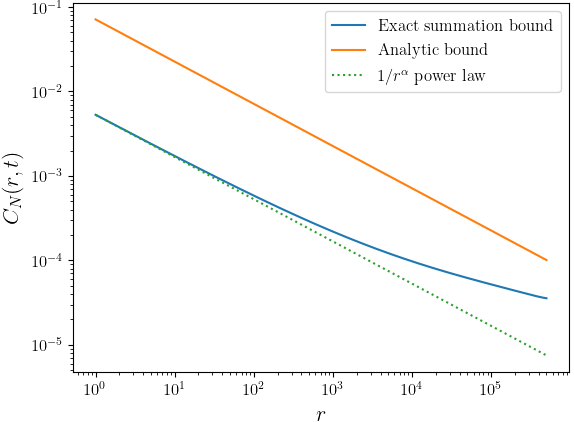
\includegraphics[width=.5\linewidth]{figures/Rdep.png}
    \caption{A comparison between the exact summation bound [\cref{eq:exactbound}] and the analytical bound [\cref{eq:newbound2}] sites as a function of the distance $r$ between operators $A$ and $B$. The specific plot assumes a 1D periodic lattice with $N = 10^6$, $\al = 0.5$, $t = 1/\lam$, and $r=1,2,\cdots,N/2$.}
    \label{Fig_Rdep}
\end{figure}

Next, we compare the $N$-dependence of the two bounds. To get rid of the $r$-dependence, we will compare the signaling times between two sites with either $r=1$ (the smallest possible separation on a 1D ring) or $r=N/2$ (the largest possible separation).
If the two bounds agree with each other at both $r=1$ and $r=N/2$ in the large $N$ limit, it is reasonable to believe that they will agree with each other at all values of $r$.

For $\al < 1$, the analytical bound gives the following signaling time (upon setting $\|[A(t),B]\|= 1$) as function of $r$ and $N$:
\begin{equation}
	\label{eq:contour_al<d}
	t_\text{si}(r,N) =\W{\frac{\log(N^{1-\al}r^{\al})}{N^{1-\al}}}.
\end{equation}
Choosing either $r=1$ or $r=N$ leads to $t_\text{si}=\Omega(N^{\al-1}\log(N))$, consistent with \cref{eq:tsi}. For the exact summation bound, we numerically compute $t_\text{si}$ by finding the value of $t$ that makes $\|[A(t),B]\| = 1$ over a range of $N$ from $10^4$ to $10^6$ for both $r = 1$ and $r = N/2$. We then fit $t$ as a function of $N$ to the function $a N^\gamma \log(N)$.
\begin{figure*}[h]
	\subfigure[~$r = 1$]{
	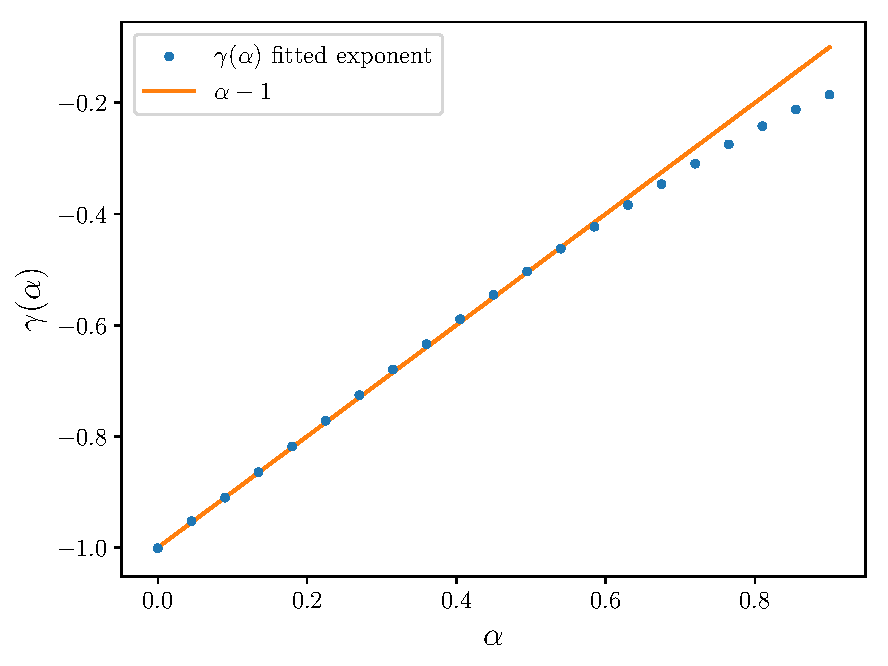
\includegraphics[width=.45\textwidth]{figures/beta_0.pdf}
    } \qquad
    \subfigure[~$r = N/2$]{
    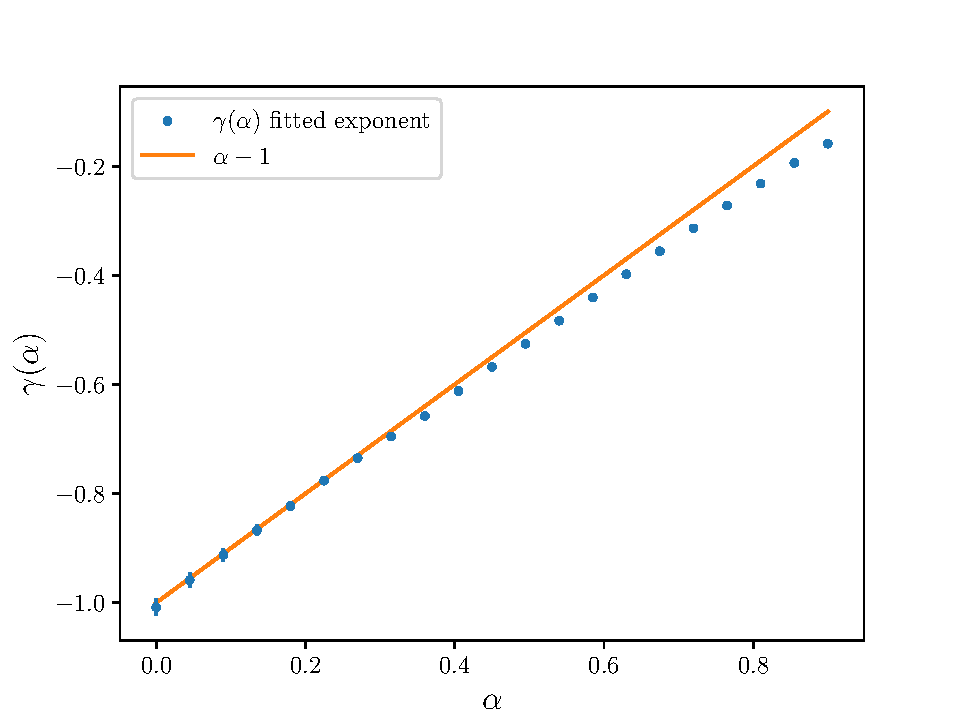
\includegraphics[width=.455\textwidth]{figures/beta_1.pdf}}
	\caption{The fitted exponent $\gamma$ in the signaling time scaling obtained from the exact summation bound in \cref{eq:exactbound} at $r=1$ (a) and $r=N/2$ (b) for $a\in [0,1]$. The error bars reflect the 95\% confidence intervals for the fit.}
        \label{Fig_al<d}
\end{figure*}
In \cref{Fig_al<d}, we plot the fitted exponent $\gamma(\al)$ as a function of $\al$. We observe that $\gamma(\al)$ scales approximately as $\al-1$ as long as $\al$ is not close to 1 for both $r=1$ and $r=N$, showing that both bounds lead to approximately the same scaling of signaling time in $N$.

When $\al\rightarrow 1$, $\gamma(\al)$ deviates from $\al-1$ noticeably. We attribute such deviation to finite-$N$ effects in our numerical evaluation of the exact summation bound. In particular, we notice that as $\al\rightarrow 1$, $\lambda$ (which plays an important role in both bounds) is not well-approximated by $N^{\al-1}$ for insufficiently large enough $N$. For such values of $N$, $\lambda$ is better approximated by $\log(N)$.

To give further clarification, we perform a comparison of the two bounds exactly at $\al=1$, where we can exactly use $\log(N)$ in place of $N^{\al-1}$. The signaling time given by the analytical bound now scales as
\begin{equation}
	t_\text{si}(r,N) = \W{\frac{\log(r\log N)}{\log N}}.\label{eq:scalinga1}
\end{equation}
We then fit the signaling time obtained from the exact summation bound at $\al=1$ using the above scaling function and find very good agreement between the two bounds. For example, at $r=1$ the signaling time from the exact summation bound can be fitted by the function $ a\:\log(N)^b\:\log\log(N)^c$ with $b=-1.0$ and $c=0.95$, which agrees with the scaling of $\log\log(N)/\log(N)$ provided by \cref{eq:scalinga1}. As a result, we expect the signaling time bounds given by both bounds to have the same scaling in $N$ when the system size is large enough for all $\al\le d$.


\singlespacing
\backmatter

% Glossary

\printbibliography[heading=bibintoc]%

% Index

\end{document}
